%\documentclass[12pt,reqno,titlepage]{book}
\documentclass[fleqn]{book}
%\usepackage{fullpage}%gives 1inch margins
\usepackage{amsmath}
\usepackage{amsthm}
\usepackage{bm}%to get bold math symbols
\usepackage[pdftex]{graphicx}
\usepackage{verbatim}
\usepackage[margin=2.5cm]{geometry}%for the margins headers footers etc
\usepackage{hyperref}%for the hyperlinks-COOL and must use
\usepackage[tt]{titlepic}%package i downloaded to put a pic in the titlepage
\usepackage{helvet}
\usepackage[usenames,dvipsnames]{color}%options to use names like redviolet and others
\usepackage{xspace}
\usepackage[mathscr]{eucal}%Defines which font to use with \mathscr
\usepackage{amssymb}%needed for \mathbb
\usepackage{enumerate}
\usepackage{comment}

%This lets you define your own style for showing the date. Below, we are defining the international standard format for dates.
\usepackage[yyyymmdd,hhmmss]{datetime}
\newdateformat{mydate}{\THEYEAR-\twodigit{\THEMONTH}-\twodigit{\THEDAY}}
\usepackage{graphicx}
%WARNING: If we instead use package ``graphics'', then this file would give an error
% Paragraph ended before \Gin@iii was complete
\graphicspath{{Figs/}}%use this to tell LaTeX where to look for images.
\usepackage{rotating} %this is what gives landscape figures

\makeatletter
\newcommand\ackname{Acknowledgements}
\if@titlepage
  \newenvironment{acknowledgements}{%
      \titlepage
      \null\vfil
      \@beginparpenalty\@lowpenalty
      \begin{center}%
        \bfseries \ackname
        \@endparpenalty\@M
      \end{center}}%
     {\par\vfil\null\endtitlepage}
\else
  \newenvironment{acknowledgements}{%
      \if@twocolumn
        \section*{\abstractname}%
      \else
        \small
        \begin{center}%
          {\bfseries \ackname\vspace{-.5em}\vspace{\z@}}%
        \end{center}%
        \quotation
      \fi}
      {\if@twocolumn\else\endquotation\fi}
\fi
\makeatother


%%%%%%%%%%%%%%%%%%%%%%%%%%%%%%%%%%%%%%%%%%%5
%\usepackage[hidelinks]{hyperref} %This is simple way to make links black. Below shows how to do it with greater control...
\usepackage{hyperref}

\definecolor{mycitecolor}{rgb}{0.4,0.15,0.15}
\definecolor{mylinkcolor}{rgb}{0.15,0.15,0.4}%dark-blue
\definecolor{myurlcolor}{rgb}{0,0,0.5}
\hypersetup{
  colorlinks   = true, %Colours links instead of ugly red boxes for cross-references and hyperlinks
  urlcolor     = myurlcolor, %Colour for external hyperlinks
  linkcolor    = mylinkcolor, %Colour of internal links
  citecolor   = mycitecolor %Colour of citations
}
\urlstyle{rm} %so it doesn't use a typewriter font for URLs.

%\url{http://ihome.ust.hk/~tanjim/verylongaddresslikethisone-111111zxzxzxzxzxzxzx
%zxzxsqut_high.pdf}
%%%%%%%%%%%%%%%%%%%%%%%%%%%%%%%%%%%%%%%%%%%5


%%%%%%%%%%%%%%%%%%%%%%%%%%%%%%%%%%%%%%%%%%%%%%%%%%%%%%% Local macros

%@@@@@@@@@@@@@@@@@@@@@@@@@@@@@
\newenvironment{MyAbstract}%
{
\leftskip=1in
\rightskip=0.5in
}
{}
%@@@@@@@@@@@@@@@@@@@@@@@@@@@@@




%%%%%%%%%%%%%%%%%%%%%%%%%%%%%%%%%%%%%%%%%%%%%%%%%%%%%%%%  From rmb_crossref.sty
\newcommand{\fig}[1]{Fig.~\ref{#1}}              % Figure
\newcommand{\eqn}[1]{Eq.~(\ref{#1})}
\newcommand{\eqs}[2]{ Eqs.~(\ref{#1}) and (\ref{#2})}
\newcommand{\Equation}[1]{Equation~(\ref{#1})}   % Equation at beg. of sentence.
%%% Usage: \showone{picture-basename}{width-fraction}
\newcommand{\showone}[2]
{%
    \begin{center}
        \includegraphics[width=#2\textwidth]{#1}%
    \end{center}
}
\newcommand{\sect}[1]{Section~\ref{#1}}          % Section

%%%%%%%%%%%%%%%%%%%%%%%%%%%%%%%%%%%%%%%%%%%%%%%%%%%%%%%% From rmb_draft.sty
\definecolor{authorNoteColor}{rgb}{.8,0,0}
\newcommand{\AuthorNote}[1]{{\color{authorNoteColor} \sffamily{\textbf{#1}}}}


%%%%%%%%%%%%%%%%%%%%%%%%%%%%%%%%%%%%%%%%%%%%%%%%%%%%%%%% From rmb_mathTypesetting.sty
\newcommand{\mathscript}[1]{%
    \ensuremath{\mathscr{#1}}%
}%
\newcommand{\scriptl}{\ell}
\newcommand{\cth}{\ensuremath{c^\text{th}}\xspace}
\newcommand{\eeth}{\ensuremath{e^\text{th}}\xspace}
\newcommand{\ith}{\ensuremath{i^\text{th}}\xspace}
\newcommand{\gth}{\ensuremath{g^\text{th}}\xspace}
\newcommand{\pth}{\ensuremath{p^\text{th}}\xspace}
\newcommand{\nth}{\ensuremath{n^\text{th}}\xspace}
\newcommand{\Vector}[1]{\ensuremath{\bm{#1}}\xspace}%
\newcommand{\Scalar}[1]{{\ensuremath{#1}}\xspace}%
\newcommand{\definedEqual}{:=}%
\newcommand{\boxit}[1]{\ensuremath{\boxed{\ensuremath{#1}}}}%
\newcommand{\by}{\ensuremath{\times}}  %The box was dimensioned 2\by3\by4
                                       %Alternative with siunitx package:
                                       %\num{2 x 3 x 4}

% usage:   \Derivpp{y}{x} will give dy/dx  with d's partials
\newcommand{\Derivpp}[2]{
        \ensuremath{\frac{\partial {#1}}{\partial {#2}}}
}

% usage:   \Derivppp{y}{x}{z} will give (dy/dx)_z partial deriv showing const
\newcommand{\Derivppp}[3]{
        \ensuremath{
          {\left(
               \frac{\partial {\ensuremath{#1}}}{\partial {\ensuremath{#2}}}
        \right)}_{\ensuremath{#3}} }
}%
\newcommand{\dd}{\mathrm{d}}

\newcommand{\Derivdd}[2]{
        \ensuremath{\frac{\dd {#1}}{\dd {#2}}}
}%
\newcommand{\Deriv}[2]{\ensuremath{\cfrac{\dd{#1}}{\dd{#2}}}}%BB



\newcommand{\Bnabla}{\ensuremath{\boldsymbol{\nabla}}}


%------------ new (not in rmb_mathTypesetting.sty
\newcommand{\aprx}[1]{\tilde{#1}}%
\newcommand{\Array}[1]{\ensuremath{\hat{\bm{#1}}}\xspace}%
\newcommand{\AArray}[1]{\ensuremath{\hat{\hat{\bm{#1}}}}\xspace}%
\newcommand{\del}{\Bnabla}


%%%%%%%%%%%%%%%%%%%%%%%%%%%%%%%%%%%%%%%%%%%%%%%%%%%%%%%% From rmb_nomenclature.sty
\newcommand{\oneD}{1-D\xspace}
\newcommand{\twoD}{2-D\xspace}
\newcommand{\threeD}{3-D\xspace}
\newcommand{\x}{\Vector{x}}
\newcommand{\Time}{\Scalar{t}}
%------------ new (not in rmb_nomenclature)
\newcommand{\NBF}{\Scalar{N}}%nodal basis function (also nodal shape function)
\newcommand{\NBFa}{\Array{N}}%nodal basis array
\newcommand{\NBFip}{\Scalar{\phi_{ip}}}%avg of \NBF_i over the \pth particle
\newcommand{\gradNBFip}{\Scalar{\Vector{G}_{ip}}}%avg of \NBF_i over the \pth particle
\newcommand{\gradNBF}{\Vector{G}}
\newcommand{\gradNBFa}{\AArray{G}}%defined in each section
\newcommand{\GBF}{\Scalar{\phi}}%grid basis function (also nodal shape function)
\newcommand{\numnodes}{\ensuremath{{\nu_\text{n}}}\xspace}%
\newcommand{\numelements}{\ensuremath{{\nu_\text{e}}}\xspace}%
\newcommand{\numgaussTotal}{\ensuremath{{\nu_\text{G}}}\xspace}% number of gauss points TOTAL
\newcommand{\numgaussOnElemente}{\ensuremath{{\nu_\text{g}(e)}}\xspace}%
\newcommand{\manuscript}{manuscript\xspace}
\newcommand{\ibase}{\Vector{i}}
\newcommand{\jbase}{\Vector{j}}
\newcommand{\kbase}{\Vector{k}}
\newcommand{\sig}{\Scalar{\sigma}}%scalar stress
\newcommand{\eps}{\Scalar{\varepsilon}}%scalar strain
%%%%%%%%%%%%%%%%%%%%%%%%%%%%%%%%%%%%%%%%%%%%%%%%%%%%%%%% From rmb_paragraphStyles.sty
%\renewcommand{\qedsymbol}{\ensuremath{\square}}
\providecommand{\qed}{........................................................}
\newcounter{example}[chapter]
  \newenvironment{example}[1][]{
    \refstepcounter{example}
    {\setlength{\leftmargin}{9cm}}%
    \subsubsection{EXAMPLE \thechapter.\arabic{example} #1}%
%\sf
    }
    {
\mbox{}
     \\
     \qed \\
    }

  \renewcommand{\theexample}{\thechapter.\arabic{example}}

\newcommand{\Bal}{\begin{aligned}}
\newcommand{\Eal}{\end{aligned}}



%%%%%%%%%%%%%%%%%%%%%%%%%%%%%%%%%%%%%%%%%%%%%%%%%%%%%%% From rmb_textStyles.sty
\definecolor{DefnColor}{rgb}{.1,.1,.6}
\newcommand{\Defn}[1]{{\color{DefnColor} {\sffamily{\textbf{#1}}}}}%
\newcommand{\eg}{\textit{e.g.,~}}
\newcommand{\ie}{\textit{i.e.,~}}
\newcommand{\cf}{\textit{cf.,~}}
\definecolor{Code}{rgb}{0,0,.6}
\newcommand{\code}[1]{{\color{Code} {\textup{\texttt{#1}}}}}
\newcommand{\etal}{\textit{et al.}\xspace}

%%%%%%%%%%%%%%%%%%%%%%%%%%%%%%%%%%%%%%%%%% From ControllingOverbarWidth.tex tutorial
\makeatletter
\newsavebox\myboxA
\newsavebox\myboxB
\newlength\mylenA
\newcommand*\xoverline[2][0.75]{%
    \sbox{\myboxA}{$\m@th#2$}%
    \setbox\myboxB\null% Phantom box
    \ht\myboxB=\ht\myboxA%
    \dp\myboxB=\dp\myboxA%
    \wd\myboxB=#1\wd\myboxA% Scale phantom
    \sbox\myboxB{$\m@th\overline{\copy\myboxB}$}%  Overlined phantom
    \setlength\mylenA{\the\wd\myboxA}%   calc width diff
    \addtolength\mylenA{-\the\wd\myboxB}%
    \ifdim\wd\myboxB<\wd\myboxA%
       \rlap{\hskip 0.5\mylenA\usebox\myboxB}{\usebox\myboxA}%
    \else
        \hskip -0.5\mylenA\rlap{\usebox\myboxA}{\hskip 0.5\mylenA\usebox\myboxB}%
    \fi}
\makeatother




%%%%%%%%%%%%%%%%%%%%%%%%%%%%%%%%%%%%%%%%%%%%%%%%%%%%%%%%%% unfiled
\newcommand{\alt}{\text{*}}
\newcommand{\gimpW}{\ensuremath{\omega}\xspace}









\begin{document}
\title{A Primer on the Material Point Method (MPM)}
\author{Rebecca Brannon}
\date{\mydate\today}
\titlepic{\setlength\fboxsep{0pt}\setlength\fboxrule{4pt}
 \fcolorbox{Plum}{green}{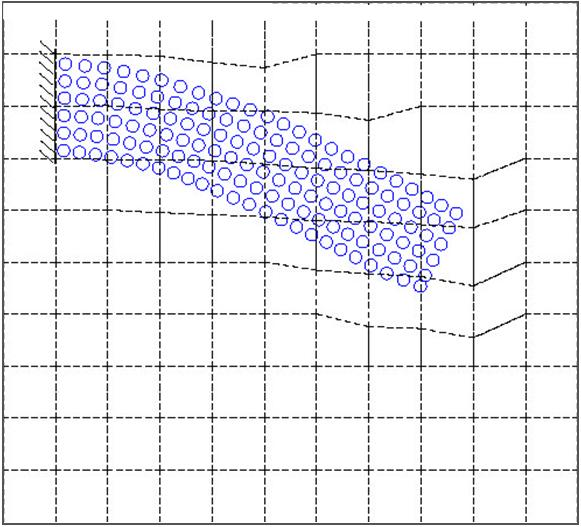
\includegraphics[width=0.3\textwidth]{CoverArtwork}}}
\begin{minipage}[h]{\textwidth}
    \maketitle
\end{minipage}
\vspace{1cm}

\begin{MyAbstract}
\paragraph{ABSTRACT:}
This \manuscript is a beginner's primer on the Material Point Method (MPM), which can be viewed as an extension of an updated-Lagrangian finite-element method (FEM) to better accommodate very complicated geometries (like intricate porous micro-structures), as well as extremely large deformations (as seen in penetration) without requiring any remapping or advection schemes for a material model's internal variables. The MPM further provides, at no additional cost, an automatic no-slip/no-stick material contact at locations not known in advance (as in compression of a porous microstructure or sloshing of a fluid).  This primer includes reviews of traditional linear FEM in \oneD, transient nonlinear FEM in \oneD and \twoD.  Following each review of traditional FEM, the revisions in the algorithm required to solve the same problem using MPM are explained.

\end{MyAbstract}






\begin{comment}
\begin{acknowledgements}
The need to write this primer became clear in August 2013, when Steve Schmidt, as student in the Computational Solid Mechanics (CSM) group at the University of Utah asked a well-known MPM researcher, Jim Guilkey, if there were any good books about the MPM.  Jim replied that he was not aware of any good books on this topic. After a pause, he added ``at least there aren't any bad books on MPM either.'' A few minutes later, Steve sent Jim a screenshot of a book advertised by Barnes and Nobel booksellers under the title ``The Material Point Method.''  Within minutes, we realized that the two Russian ``authors'' were known to farm Wikipedia to create ``books'' that they didn't write themselves.  Therefore, thanks go to Barnes and Nobel for their failure to filter out this sort of sleazy publishing, prompting us to try writing an MPM book!
\end{acknowledgements}
\end{comment}

\chapter{A Primer on the Material Point Method (MPM)}
\begin{comment}
This \manuscript is a tutorial on the Material Point Method (MPM). The goal is to show you how to write your own MPM code assuming that you already have an FEM code available to modify, or at least can write one as needed. This tutorial does not explain syntax of any particular MPM code. 

A brief review of the finite-element method (FEM) is provided to establish notational choices made in this \manuscript and to form a starting point from which revisions are applied to convert an FEM code to an MPM code.  This review of FEM uses notation from \threeD problems with the expectation that the reader knows how to modify the discussion appropriately for lower-dimension problems. Following the broad review of FEM, this manuscript then summarizes specific FEM formulations for \oneD and \twoD problems, showing what revisions are needed to convert the FEM solver to an MPM solver.


\section{A review of FEM}
The reader is assumed to be familiar with the finite-element method (FEM), so this section is primarily focused on defining our notational preferences. 

\subsection{FEM grid, elements, nodes, and shape functions}
An FEM solution to a differential equation begins by introducing a body-fitted grid that tessellates the spatial domain into \Defn{elements}.\footnote{A \Defn{tesselation} breaks up a physical domain, here called a \Defn{body}, into a set of subdomains without gaps or overlaps.} 
%
In \twoD, some FEM codes break the body into quadrilateral elements, while other FEM codes use triangles (see \fig{fig:QuadAndTriangleMesh}). Higher-order methods use increasingly complicated shapes, but all choices have in common that the element shape is determined from special points on the element called \Defn{nodes}. The reader is presumed to be very comfortable working with nodes, elements, and \Defn{connectivity} (\ie the mapping of local node numbers on an element to/from global node numbers on the mesh).





\begin{figure}
\showone{QuadAndTriangleMesh}{1.0}
\caption{(a)quadrilateral mesh (b)triangle mesh. Image permission still needed from \cite{Khoei2008}}
\label{fig:QuadAndTriangleMesh}
\end{figure}



%
The reader is further expected to know that, associated with the \ith node is a spatially varying the \Defn{nodal basis function} $\NBF_i(\x)$ (also called the \Defn{shape function}\footnote{Purists use the term \Defn{shape function} to refer to the function defined on an element, while \Defn{nodal basis function} is defined on the entire domain. Thus, for example, several different linear shape functions are used to construct the single classic ``tent'' nodal basis function, which certainly is not linear -- it is piecewise linear! We will make no such distinction between \textit{shape function} and \textit{nodal basis function}, as the intended meaning is always clear from context.}), such that a discretized approximation of a field $f(\x,\Time)$, which varies with position \x and time \Time, is\footnote{Here and throughout this primer, broadly applicable equations will be given in their general form for transient \threeD problems, where \x denotes the position vector and \Time is time. The reader is expected to know how to revise these formulas for special case situations such as \oneD problems (where $x$ is just a scalar) and/or for statics problems (where dependence on time is absent). Most of the upcoming examples will be limited to \oneD and \twoD problems for clarity.}


\begin{equation}
  \aprx{f}(\x,\Time)=\sum\limits_{i=1}^{\numnodes} \aprx{f}_i(\Time) \NBF_i(\x)
\label{eq:fieldOnGridc}
\end{equation}
{\samepage{
where a tilde $(\sim)$ is used to distinguish between an exact field $f$ and its approximation $\aprx{f}$. The summation over $i$ varies over the number of nodes \numnodes, and $\aprx{f}_i(\Time)$ is the time-varying \Defn{nodal value} of the approximate field associated with the \ith node, having a position vector denoted $\x_i$.\footnote{which might or might not be equal to the actual field $f(\x,t)$ at that node.}  The above expansion is called an \Defn{interpolation} if the shape functions satisfy
\begin{equation}
\boxit{
 \quad \text{\Defn{Kronecker property:}}\qquad
\NBF_i(\x_j)=\delta_{ij}=\begin{cases}
                                1 &\text{ if }i=j
                                \\
                                0 & \text{ if }i\ne j
                         \end{cases}
\quad}
\end{equation}
}}
The Kronecker property ensures that $\aprx{f}_i(\Time)=\aprx{f}(\x_i,\Time)$, but not necessarily \mbox{$\aprx{f}_i(\Time)=f(\x_i,\Time)$,} where (recall) $f(\x,t)$ is the exact function and $\aprx{f}(\x,t)$ is its approximation. In fact, as illustrated in \fig{fig:LinearFitNotInterpolation}, the best fit might not be an interpolation to that function -- it depends on how you define error!

\begin{figure}
\showone{InterpolationContrastedWithMinSquareError}{0.8}
\caption{Exact function $f(\x,t)$ and two choices for a piecewise linear fit $\aprx{f}(\x,t)$, differing only by the choice of nodal values $\aprx{f}_i(t)$. (a) Best five-node piecewise-linear fit to a function when ``best'' corresponds to minimizing nodal errors; in this case, the nodal values exactly match the function values at the nodes: $\aprx{f}_i(\Time)=f(x_i,\Time)$. (b) Best piecewise-linear fit when the goal is instead to minimize overall mean square error; in this case $\aprx{f}_i(\Time)\ne f(x_i,\Time)$.  In both graphs, dashed lines correspond to element boundaries. The piecewise linear fits (in red) use standard linear shape functions $\NBF_i(x)$, which therefore correspond to ``tent'' nodal basis functions that are often used in FEM analyses.}
\label{fig:LinearFitNotInterpolation}
\end{figure}

Many FEM textbooks introduce a compact notation for the collection of shape functions and nodal values. Let $\NBFa(\x)$ denote the column array containing the shape functions:
\begin{equation}
  \NBFa(\x)\definedEqual
{\begin{bmatrix}\NBF_1(\x) \\ \NBF_2(\x)  \\ \vdots  \\  \NBF_\numnodes(\x) \end{bmatrix}}
\qquad\text{and therefore}\qquad
\NBFa^T(\x)=[\NBF_1(\x),\NBF_2(\x),\ldots,\NBF_\numnodes(\x)]\;.
\label{eq:ArrayNBFa}
\end{equation}
If we similarly define $\Array{f}\definedEqual[\aprx{f}_1,\ldots,\aprx{f}_\numnodes]^T$, the matrix versions of \eqn{eq:fieldOnGridc} are then
\begin{equation}
  \aprx{f}(\x,\Time)=\NBFa^T(\x)\Array{f}(t)=\Array{f}^T(t)\NBFa(\x)\;.
\label{eq:fieldOnGrida}
\end{equation}
This notation will be adopted later when analyzing the weak form of the governing equations. 

The Kronecker property is not required for a nodal basis function to provide an acceptable numerical approximation to a field. We will, however, require the nodal basis function to satisfy:
\begin{equation}
  \boxit{\quad
\text{\Defn{Partition of unity: }}\quad
\sum\limits_{i=1}^{\numnodes} \NBF_i(\x)\equiv 1\qquad\forall\x
\quad}
\label{eq:PartitionOfUnity}
\end{equation}
When this property holds, $\aprx{f}(\x,t)$ can be made to exactly represent a constant field by simply selecting each $\aprx{f}_i$ to equal that constant. 
The following \textit{additional} property is needed to exactly represent a field that varies linearly in space:
\begin{equation}
  \boxit{\quad
\text{\Defn{Linearly complete: }}\quad
\sum\limits_{i=1}^{\numnodes} \x_i\NBF_i(\x)\equiv \x\qquad\forall\x
\quad}
\label{eq:LinearlyComplete}
\end{equation}




\subsubsection{What is the finite-element method, really?}
In order to declare that a numerical solver is using the finite-element method, we assert that each nodal basis function must have all of the following properties:
\begin{enumerate}[i.]
  \item The body must be tesselated into subdomains called elements. To be a tesselation, the elements must not overlap each other, and their union must represent an approximation of the body without gaps.  Moreover, the elements must be constructed in a systematic way from discrete points on or inside the body, called nodes, such that each element is formed from a finite set of nodes. Generally one node is used to form multiple elements. Any two elements that share a node are said to be \Defn{neighboring elements}.
  \item A field $f(\x,\Time)$ must be approximated by $\aprx{f}(\x,\Time)\definedEqual\sum\limits_1^\numnodes \aprx{f}_i(\Time) \NBF_i(\x)$.
  \item Each $\NBF_i(\x)$ must be associated with nodes on tesselation domains (elements) and be nonzero only over the.
  \item Each $\NBF_i(\x)$ must satisfy the Kronecker property:  $\NBF_i(\x_j)=\delta_{ij}$
  \item Each $\NBF_i(\x)$ must satisfy partition of unity: $\sum\limits_{i=1}^{\numnodes} \NBF_i(\x)\equiv 1\qquad\forall\x$
  \item Each $\NBF_i(\x)$ must be linearly complete: $\sum\limits_{i=1}^{\numnodes} \x_i\NBF_i(\x)\equiv \x\qquad\forall\x$
\end{enumerate}














\subsubsection{FEM notation for the gradient of a scalar field}
Let $x$, $y$, and $z$ denote the \Defn{Cartesian components of the position vector} \x.  Let $\ibase$, $\jbase$, and $\kbase$ be the associated \Defn{unit basis vectors}.
Let $s(\x,\Time)$ denote a scalar-valued function of position \x and time \Time. The gradient of this field is a vector defined by
\begin{equation}
  \Derivpp{s}{\x}=\del s
=\Derivpp{s}{x}\ibase
+\Derivpp{s}{y}\jbase
+\Derivpp{s}{z}\kbase
\end{equation}
Applying this definition to the expansion in \eqn{eq:fieldOnGridc} gives
\begin{equation}
  \Derivpp{\aprx{f}}{\x}=\sum\limits_{i=1}^{\numnodes} \aprx{f}_i(\Time) \gradNBF_i(\x)
\qquad\text{where}\qquad
\gradNBF_i(\x)\definedEqual\Derivpp{\NBF_i}{\x}
\label{eq:gradfieldOnGridc}
\end{equation}
Equivalently, using the ``nabla'' (del) notation,
\begin{equation}
  \del\aprx{f}(\x,\Time)=\sum\limits_{i=1}^{\numnodes} \aprx{f}_i(\Time) \gradNBF_i(\x)
\qquad\text{where}\qquad
\gradNBF_i(\x)\definedEqual\del\NBF_i(\x)
\label{eq:delfieldOnGridc}
\end{equation}

Let us now introduce a matrix $\gradNBFa$ whose \ith row contains the components of the gradient of the \ith shape function:
\begin{equation}
  \gradNBFa\definedEqual
\begin{bmatrix}
\Derivpp{\NBF_1}{x} & \Derivpp{\NBF_1}{y} & \Derivpp{\NBF_1}{z} \\
\Derivpp{\NBF_2}{x} & \Derivpp{\NBF_2}{y} & \Derivpp{\NBF_2}{z} \\
                 & \vdots           &                  \\
\Derivpp{\NBF_\numnodes}{x} & \Derivpp{\NBF_\numnodes}{y} & \Derivpp{\NBF_\numnodes}{z} \\
\end{bmatrix}
\end{equation}
Recalling that $\Array{f}$ denotes the \numnodes\by1 array containing nodal values of the field, the matrix notation for \eqn{eq:gradfieldOnGridc} is
\begin{equation}
  \underset{1\by3}{\Derivpp{\aprx{f}}{\x}}= 
\underset{1\by\numnodes}{\Array{f}^T(\Time)}
\underset{\numnodes\by3}{\gradNBFa(\x)}
\label{eq:gradfieldOnGridcMatrixA}
\end{equation}
or, taking the transpose of both sides,
\begin{equation}
  \underset{3\by1}{\Derivpp{\aprx{f}}{\x}}= 
\underset{3\by\numnodes}{\gradNBFa^T(\x)}
\underset{\numnodes\by1}{\Array{f}(\Time)}
\label{eq:gradfieldOnGridcMatrixB}
\end{equation}
Here, the undersets show the dimensions of each matrix for clarity. Since $\del f$ is a physical vector having three components, the above two equations clarify that these components may be arranged as either a 3\by1 or 1\by3 array.

\subsection{FEM notation for vector fields and their gradients}
Let $\Vector{u}=u_x \ibase + u_y \jbase + u_z \kbase$ denote a generic vector (like displacement) in \threeD.  Suppose that this generic vector is a field, $\Vector{u}(\x,\Time)$, which is described approximately in terms of the basis functions by
\begin{equation}
  \aprx{\Vector{u}}(\x,\Time)\approx\sum\limits_{i=1}^{\numnodes} \aprx{\Vector{u}}_i(\Time) \NBF_i(\x)
\label{eq:vecfieldOnGridc}
\end{equation}
%
We define the \threeD component array for the left-hand side of this equation vector using a ``single hat'' notation:
\begin{equation}
  \Array{u}(\x,\Time)\definedEqual\begin{bmatrix}
                               \aprx{u}_x(\x,\Time) \\ 
                               \aprx{u}_y(\x,\Time) \\ 
                               \aprx{u}_z(\x,\Time)
                        \end{bmatrix}
\end{equation}
For each node, there is an associated nodal vector $\Vector{\aprx{u}}_i(\Time)$.  This \manuscript will use a DOUBLE-hat notation to refer to the \numnodes\by3 matrix whose \ith row contains the three components $\Vector{u}_i$. That is,
\begin{equation}
  \AArray{u}(\Time)\definedEqual
\begin{bmatrix}
\aprx{u}_{1x}(\Time) & \aprx{u}_{1y}(\Time) &  \aprx{u}_{1z}(\Time) \\
\aprx{u}_{2x}(\Time) & \aprx{u}_{2y}(\Time) &  \aprx{u}_{2z}(\Time) \\
              &     \vdots    &                \\
\aprx{u}_{\numnodes x}(\Time) & \aprx{u}_{\numnodes y}(\Time) &  \aprx{u}_{\numnodes z}(\Time)
\end{bmatrix}
\end{equation}
Thus, recalling that \eqn{eq:ArrayNBFa}, the matrix form of \eqn{eq:vecfieldOnGridc} is
\begin{equation}
  \Array{u}=\AArray{u}^T(\Time)\NBFa(\x)
\end{equation}


As a special case, let $\Array{x}$ denote the component array of the position vector \x, and let $\AArray{x}$ denote the matrix of node locations as follows:
\begin{equation}
  \Array{x}\definedEqual\begin{bmatrix}
                               x \\ 
                               y \\ 
                               z
                        \end{bmatrix}
\qquad\text{and}\qquad
  \AArray{x}\definedEqual
\begin{bmatrix}
x_{1} & y_{1} &  z_{1} \\
x_{2} & y_{2} &  z_{2} \\
              &     \vdots    &                \\
x_{\numnodes} & y_{\numnodes} &  z_{\numnodes}
\end{bmatrix}
\end{equation}
Then the matrix form of \eqn{eq:LinearlyComplete} is
\begin{equation}
  \boxit{\quad
\text{\Defn{Linearly complete: }}\quad
\Array{x}=\AArray{x}^T\NBFa(\x)
\quad}
\label{eq:highDimLinearlyComplete}
\end{equation}

\subsubsection{Gradients of vector fields}
The gradient of a generic vector field $\Vector{u}(\x,\Time)$ is a second-order tensor, denoted $\partial\Vector{u}/\partial\x$, having a 3\by 3 component matrix given by
\begin{equation}
\left[\Derivpp{\Vector{u}}{\x}\right]\definedEqual
\begin{bmatrix}
\Derivpp{u_x}{x} & \Derivpp{u_x}{y} & \Derivpp{u_x}{z} \\
\Derivpp{u_y}{x} & \Derivpp{u_x}{y} & \Derivpp{u_y}{z} \\
\Derivpp{u_z}{x} & \Derivpp{u_z}{y} & \Derivpp{u_z}{z}
\end{bmatrix}
\end{equation}
Applying this definition, the gradient of the \emph{approximate} vector field is evaluated by the matrix multiplication



\begin{equation}
  \underset{3\by3}{\Derivpp{\aprx{\Vector{u}}}{\x}}= 
\underset{3\by\numnodes}{\AArray{u}^T(\Time)}
\underset{\numnodes\by3}{\gradNBFa(\x)}
\label{eq:gradfieldOnGridcMatrixC}
\end{equation}








\newpage
description of the field  described by using nodal basis functions (also called element shape functions\footnote{Purists prefer the phrase \Defn{element shape function} to refer to the function that applies on an element, while the nodal basis function applies over the entire domain. Thus, for example, a linear shape function has the equation of a straight line, but the nodal basis function is the assembly of shape functions into the form of a so-called ``tent function,'' which is certainly not linear -- it is piecewise linear.}) and nodal values mapping from discrete  on the FEM grid to any 

,  more generally any convex polygon, to represent particle domains, which more accurately represents the boundary and thus gives lower errors on the same mesh resolution.  In both (a) and (b), note that the particle density is generally
\begin{figure}
\showone{CPDIstairSteppingGeometry}{0.7}
\label{fig:CPDIstairSteppingGeometry}
\caption{MPM particles (small hollow circles) distributed within an overlaid rectilinear grid (dashed lines). The rectangles around the particles represent the physical domain of material occupied by each particle. (a) A pixelated description of an angled beam has a jagged (stair-stepped) boundary, which will give errors in an MPM simulation that would be comparable to using FEM with the same jagged mesh. (b) So-called ``conforming'' particle domains, are shown here as tilted rectangles, and these might be more complicated convex polygons in more complicated geometries.}
\end{figure}












Because this tutorial treats MPM as an extension of the finite-element method, you should be able to convert an existing conventional FEM code to an MPM code without much difficulty.\footnote{At Sandia National Laboratories, for example, a mature FEM code was converted to MPM in only one week, and simulations were run and visualized only a week after that.} Some reasons to add an MPM option to an FEM code are:
\begin{itemize}
\item Simulations can be run on complicated geometries, such as intricate porous structures, without the need for difficult material-based nodal connectivity tables that are used in conventional FEM to track material adjacent to any given element. 
\item The geometry for an MPM simulation can be initialized directly from voxel information from a computed tomography (CT) scan.\footnote{A voxel is the \threeD analog of a pixel in \twoD.} A voxel-based representation of a body treats the body as a collection of cuboids, somewhat like a Lego model of a structure. Such a representation is possible with both FEM and MPM (each having comparable errors caused by poor description of angled boundaries, such as those evident in \fig{fig:CPDIstairSteppingGeometry}), so the real advantage of MPM is that it does not require defining \emph{material} connectivity information. Accordingly, an update to connectivity is not required to model subsequent material fracture.
\item With MPM, the governing equations may be solved on a simple rectilinear grid, rather than requiring the body-fitted meshes used in traditional FEM.\footnote{Optionally, a body-fitted mesh may still be used to define the body in MPM while simultaneously using a simple overlaid rectilinear grid for the field equations, and doing so can significantly improve MPM accuracy.  Furthermore, a non-rectilinear mesh may be used with the MPM, but doing so entails additional computational cost.}
\item FEM formulations save material constitutive data at Gauss points with displacement, velocity, and acceleration at nodes.  Under conditions of extremely large deformations, an FEM formulation must remesh to remove excessive element distortion. This process of remeshing then must be followed by remapping of the material constitutive data to the new locations of Gauss points. The remapping phase (which is essentially an averaging process) results in so-called \emph{advection} errors that can corrupt the physical meanings of material constitutive model data.\footnote{For example, mixing stress states in a plasticity model model might produce a new stress state violating the yield condition of the model. A fiber composite model that has the fiber direction (a unit vector) saved as a constitutive internal variable, then attempting to average these directions generally produces a vector that is no longer of unit length. While ad hoc workarounds can be usually found to assign physically admissible rezoned constitutive variables, those methods are rarely robust and certainly not defensible from a physical standpoint. The efforts to find workarounds for advection errors are so time consuming that it is far better to implement new methods, like MPM, that eliminate the need for advection corrections altogether.}  An MPM formulation saves all field variables (constitutive and kinematic) at material particles. These particles represent the body and flow through the overlaid grid, carrying all of their particle data with them. When an FEM code is revised to become an MPM code, the key algorithm adjustment is the insertion of a phase that maps data from particles to grid to solve the governing differential equations on the grid, followed by a mapping of the solution from the grid to particles to finish updating the state.  Because MPM formulations save data at particles, and because those particles may flow an arbitrary distance through the overlaid mesh, the MPM can model very large deformations without any advection errors. 
\end{itemize}
\end{comment}



\newpage
\newcommand{\tractionForce}{\mathscript{F}}
\section{The classic starting point: linear quasistatic \oneD bar problem}
This section provides a ``learn by example'' introduction to the Material Point Method (MPM) by showing how to solve the classical quasi-static uniaxial bar equation,
\begin{equation}
\Bal
  &\frac{\dd~~}{\dd x}\left[E(x)A(x) \frac{\dd u(x)}{\dd x~~~}\right]+f(x)=0 \qquad  &          &\text{on domain $\Omega$ defined by }0<x<L& \\
  &\text{subject to Robin BCs: }
       &&\alpha_0 \tractionForce(0)+\beta_0 u(0)=\gamma_0 \\
       &&\text{and ~~}&\alpha_L \tractionForce(L)+\beta_L u(L)=\gamma_L 
\Eal
\label{eq:LinearBarStrongForm}
\end{equation}
Here, $E(x)$ is the bar stiffness,\footnote{The modulus $E$ is commonly thought to be equal to Young's modulus, which is true for uniaxial stress (where the lateral stress is zero), but it is actually a different modulus, called the constrained modulus, if the loading is uniaxial strain (where the lateral strain is zero)} 
%
$A(x)$ is the cross-sectional area of the bar, 
%
$f(x)$ is the spatially varying distributed load on the bar\footnote{The distributed load has dimensions of force per unit length. Point loads are accommodated by allowing the distributed load to include Dirac delta contributions.}, 
%
and $u(x)$ is the displacement.  
%
In the Robin boundary conditions, 
\begin{equation}
  \tractionForce(0)\definedEqual -E(0)A(0)u'(0)
\qquad\text{and}\qquad
  \tractionForce(L)\definedEqual  E(L)A(L)u'(L)
\label{eq:boundaryForces}
\end{equation}
are the forces at the left and right ends of the bar, respectively (each defined to be positive when pointing to the right, which is why the first one is defined with a negative). The Robin parameters, $\alpha_0,~\beta_0,~\gamma_0,~\alpha_L,~\beta_L, \text{ and } \gamma_L$, are user-prescribed constants. 
These conditions include the following special cases:
%
prescribed displacement,\footnote{found by setting the $\alpha$ parameter to zero, $\beta=1$, and $\gamma$ equal to the prescribed displacement}
%
prescribed force,\footnote{by setting $\alpha=1$, $\beta=0$, and $\gamma$ equal to the precribed force}
%
and a spring BC.\footnote{found by setting $\alpha=1$, $\beta$ equal to the negative of the spring constant}

This section is broken into four subsections. First, the governing equation is recast as an integral equation to lessen the differentiability requirements of approximate solutions. Next, the traditional FEM solution is provided, and then it is converted to an MPM formulation. This section finishes with a step-by-step MPM algorithm.  Subsequent sections build up from this simple \oneD bar problem to allow material nonlinearity, first in \oneD and then in \twoD.

\subsection{The weak form of the governing equation}
The ODE in \eqn{eq:LinearBarStrongForm} is called the \Defn{strong form} of the governing equation, which requires the displacement function $u(x)$\footnote{The  displacement function is often called called the \Defn{trial function}, which is an abstraction introduced to emphasize that this same ODE applies to many more physical applications than just motion of an elastic bar.} to have no jumps in slope (no cusps) in order to be twice differentiable.  The strong form is then multiplied by an arbitrary weight function\footnote{In variational formulations, the function $w(x)$ is called the \Defn{test function}, and it is interpreted physically as a small perturbation of the displacement (often denoted $\delta u(x)$).  Variational formulations of the finite-element method often state that the test function $w(x)$ is required to vanish on the parts of the boundary where the trial function $u$ is specified, but this restriction is NOT actually needed, so we will not adopt it in this work.} $w(x)$, and then integrated over the domain from $x=0$ to $x=L$:
\begin{equation}
  \int\limits_0^L w(x) \frac{\dd~~}{\dd x}\left[E(x)A(x) \frac{\dd u(x)}{\dd x~~~}\right]\dd x  +  \int\limits_0^L w(x)f(x)\dd x=0
\qquad\forall w(x)
\end{equation}
The first term is integrated by parts\footnote{Namely, $\int_0^L u \Derivdd{v}{x} dx = uv \big|_0^L-\int_0^L u \Derivdd{v}{x} dx$. In this case the \emph{entire} expression in the brackets, $\left[E(x)A(x) \frac{\dd u(x)}{\dd x~~~}\right]$ is taken as the quantity ``$v$'', and $w(x)$ is taken as ``$u$''.}  to give the so-called \Defn{weak form} of the governing equation:
\begin{equation}
  E(x)A(x) w(x)u'(x)\big|_0^L-\int\limits_0^L EA w'(x)u'(x)\dd x  +  \int\limits_0^L w(x)f(x)\dd x=0
\qquad\forall w(x)
\label{eq:LinearBarWeakForm}
\end{equation}
Using the definition of boundary forces defined in \eqn{eq:boundaryForces}, this may be written
\begin{equation}
 \int\limits_0^L E(x)A(x) w'(x)u'(x)\dd x = w(0)\tractionForce(0)+w(L)\tractionForce(L)  +  \int\limits_0^L w(x)f(x)\dd x=0
\qquad\forall w(x)
\label{eq:LinearBarWeakFormWithForcesc}
\end{equation}
This is called the ``weak'' form of the governing equation because the trial function, displacement $u(x)$, now has only one derivative on it. This will allow us to seek approximate solutions that are merely continuous rather than needing to find functions that have continuous slopes.




\subsection{Traditional FEM formulation of the bar problem}
\label{sec:LinearBarFEM}
A traditional FEM solution to any \oneD problem begins by introducing a set of nodes, which are points distributed along the length of the bar (assumed to be numbered sequentially from 1 to \numnodes, where \numnodes denotes the total number of nodes).  The nodes are furthermore used to define elements on the finite-element mesh, as explained in any introductory FEM textbook.  Below \numelements denotes the total number of elements.
 
The approximate FEM solution for the displacment field is
\begin{equation}
  \aprx{u}(x)\definedEqual\sum\limits_{j=1}^{\numnodes}\aprx{u}_j \NBF_j(x)
\label{eq:aprxuc}
\end{equation}
where $\{\NBF_1(x),\NBF_2(x),\ldots,\NBF_\numnodes\}$ are the nodal basis functions (such as the ``tent'' functions constructed from linear shape functions), and $\{\aprx{u}_1, \aprx{u}_1, \ldots, \aprx{u}_\numnodes\}$  
are the nodal displacements.\footnote{The reader is presumed to be familiar enough with the finite-element method that these statements require no detailed explanations or clarification.}

The weight function in the weak formulation is similarly expanded as
\begin{equation}
  w(x)\definedEqual\sum\limits_{i=1}^{\numnodes}w_i \NBF_i(x)
\label{eq:weightc}
\end{equation}

In the finite-element method, the nodal basis functions are required to satisfy the following properties:

\begin{subequations}
\begin{align}
\text{\Defn{Kronecker property:}}\qquad&
\NBF_i(x_j)=\delta_{ij}=\begin{cases}
                                1 &\text{ if }i=j
                                \\
                                0 & \text{ if }i\ne j
                         \end{cases}
\label{eq:oneDRequirementsOnShapeFnsKronecker}
\\
\text{\Defn{Partition of unity:}}\qquad&
\sum\limits_{i=1}^\numnodes \NBF_i(x)=1     \qquad\forall x
\\
\text{\Defn{Linear completeness:}}\qquad&
\sum\limits_{i=1}^\numnodes x_i\NBF_i(x)=x     \qquad\forall x
\\
\text{\Defn{FEM compact support:}}\qquad&
\NBF_i(x)=0 \qquad\forall x 
\text{ falling in an element not including node $i$}
\label{eq:oneDRequirementsOnShapeFnsFEMsupport}
\\
\text{\Defn{Weak-form integrability:}}\qquad&
\NBF_i(x)\text{ must be continuous}
\label{eq:oneDRequirementsOnShapeFnsFEMcontinuity}
\end{align}
\label{eq:oneDRequirementsOnShapeFns}
\end{subequations}
As explained in any good introductory FEM textbook, the last condition imposes the requirement implied from the weak formulation that we must seek solutions that are continuous.

\renewcommand{\gradNBFa}{\Array{G}}
Let $\NBFa(x)$ denote a 
$\numnodes\by1$ column array of the nodal basis functions. For future use, let $\gradNBFa$ denote the array of spatial gradients of the nodal basis functions. Similarly, 
let $\Array{u}$ and $\Array{w}$ denote \numnodes\by1 column arrays of nodal displacements and nodal weights, respectively:
\begin{equation}
  \NBFa(x)\definedEqual\begin{bmatrix}\NBF_1(x)\\ \NBF_2(x) \\ \vdots \\ \NBF_\numnodes(x)\end{bmatrix}
\qquad\qquad
  \gradNBFa(x)\definedEqual\begin{bmatrix}\NBF_1'(x)\\ \NBF_2'(x) \\ \vdots \\ \NBF_\numnodes'(x)\end{bmatrix}
\qquad\qquad
  \Array{u}\definedEqual\begin{bmatrix} \aprx{u}_1\\ \aprx{u}_2 \\ \vdots \\ \aprx{u}_\numnodes\end{bmatrix}
\qquad\qquad
  \Array{w}\definedEqual\begin{bmatrix}w_1\\ w_2 \\ \vdots \\ w_\numnodes\end{bmatrix}
\end{equation}

Then \eqs{eq:aprxuc}{eq:weightc} may be written in matrix form as\footnote{Commutativity of scalar multiplication allows us to put the nodal basis array either on the left (with a transpose) or on the right (without transpose) as done here. In anticipation of upcoming parts of the analysis, we find it convenient to have the displacement array placed on the right with the weight array on the left.}
\begin{equation}
  \aprx{u}(x)=\underbrace{
\underbrace{\NBFa^T(x)}_{1\by\numnodes} \underbrace{\Array{u}}_{\numnodes\by1}}_{1\by1}
\qquad\text{and}\qquad
  w(x)=\underbrace{\underbrace{\Array{w}^T}_{1\by\numnodes}\underbrace{\NBFa(x)}_{\numnodes\by1}}_{1\by1}
\end{equation}
The superscript ``T'' denotes the transpose, which turns a column array into a row array and hence reverses the matrix dimensions as indicated.  The end result is a 1\by1 matrix, which is simply a single number.  Let us also define a ``reaction array'' $\Array{\tractionForce}$ having all zero components except in the first and last components as follows:
\begin{equation}
  \Array{\tractionForce}\definedEqual
\begin{bmatrix}
\tractionForce(0) \\
0 \\
0 \\
\vdots\\
0 \\
0 \\
\tractionForce(L)
\end{bmatrix}
\qquad\text{which allows writing }\qquad
w(0)\tractionForce(0)+w(L)\tractionForce(L)=\Array{w}^T\Array{\tractionForce}
\end{equation}
Making these substitutions into \eqn{eq:LinearBarWeakFormWithForcesc} gives
\begin{equation}
 \int\limits_0^L E(x)A(x) 
\underbrace{
	\underbrace{
           \Array{w}^T
   }_{1\by\numnodes}
	\underbrace{
	      \underbrace{
              \gradNBFa(x)
          }_{\numnodes\by1}
	     \underbrace{
            \gradNBFa^T(x)
          }_{1\by\numnodes}
	}_{\numnodes\by\numnodes}
	\underbrace{\Array{u}}_{\numnodes\by1}
}_{1\by1} 
\dd x 
= 
\underbrace{\underbrace{\Array{w}^T}_{1\by\numnodes}\underbrace{\Array{\tractionForce}}_{\numnodes\by1}}_{1\by1}
+  \int\limits_0^L \underbrace{\underbrace{\Array{w}^T}_{1\by\numnodes}\underbrace{\NBFa(x)}_{\numnodes\by1}}_{1\by1}f(x)
\dd x
 \qquad\forall\Array{w}
\label{eq:LinearBarWeakFormWithForces}
\end{equation}
where (recall) $\gradNBFa(x)$ denotes the array of shape function gradients,

Since this must hold $\forall\Array{w}$, the premultiplication by $\Array{w}^T$ may be removed. Also, recognizing that $\Array{u}$ does not vary with $x$, it may be removed from the first integral, giving
\begin{equation}
\AArray{K}\Array{u}
=
\Array{\tractionForce}  
+  \Array{f}
\label{eq:LinearBarWeakFormDiscr}
\end{equation}
where
\begin{equation}
\boxit{\quad
\text{\Defn{Global Stiffness:}}\quad
  \underbrace{\AArray{K}}_{\numnodes\by\numnodes}\definedEqual\int\limits_0^L E(x)A(x)  \underbrace{\underbrace{\gradNBFa(x)}_{\numnodes\by1} \underbrace{\gradNBFa^T(x)}_{1\by\numnodes}}_{\numnodes\by\numnodes} \dd x
\quad}
\label{eq:linearBarGlobalStiffness}
\end{equation}
and
\begin{equation}
\boxit{\quad
\text{\Defn{Body force array:}}\quad
  \underbrace{\Array{f}}_{\numnodes\by1}
\definedEqual
\int\limits_0^L f(x)\underbrace{\NBFa(x)}_{\numnodes\by1}\dd x
\quad}
\label{eq:linearBarBodyForceArray}
\end{equation}

\subsubsection{Counting unknowns and equations to confirm solvability}
\Equation{eq:LinearBarWeakFormDiscr} represents a set of \numnodes equations involving $\numnodes+2$ unknowns: 
\begin{equation}
 \text{\Defn{A total of $\numnodes+2$ unknowns}:}\qquad u_1, u_2, \ldots, u_\numnodes,\quad \tractionForce(0), \tractionForce(L)
\end{equation}
Not only are the nodal displacements unknown, so are the boundary forces, $\tractionForce(0)$ and $\tractionForce(L)$, located at the first and last components of $\Array{\tractionForce}$.  To achieve a solvable system, \eqn{eq:LinearBarWeakFormDiscr} must be supplemented with the two boundary conditions in \eqn{eq:LinearBarStrongForm}.  Namely, noting that $u(0)=u_1$ and $u(L)=u_\numnodes$,
\begin{equation}
\Bal
\alpha_0 \tractionForce(0)+\beta_0 u_1&=\gamma_0 \\
\alpha_L \tractionForce(L)+\beta_L u_\numnodes&=\gamma_L 
\Eal
\label{eq:LinearBarStrongFormBCs}
\end{equation}
Together, \eqs{eq:LinearBarWeakFormDiscr}{eq:LinearBarStrongFormBCs} form a set of $\numnodes+2$ equations solvable for the $\numnodes+2$ unknowns!  Specific methods of solution, covered in a first course on the finite-element method, are not discussed in this \manuscript.

\subsubsection{FEM integral evaluation}
In the finite-element method, a large fraction of the work goes into evaluation of the integrals in \eqs{eq:linearBarGlobalStiffness}{eq:linearBarBodyForceArray}.  Since there are two integrals to be evaluated, let's discuss them generically by letting $\zeta(x)$ denote the integrand so that the task is to evaluate 
\begin{equation}
  \int\limits_\Omega \zeta(x) \dd x
\label{eq:LinearBarGenericIntegral}
\end{equation}
where $\Omega$ represents the integration domain spanning from $x$=$0$ to $x$=$L$. For the stiffness integral, the integrand is $\zeta(x)=E(x)A(x)\gradNBFa(x)\gradNBFa^T(x)$. For the force integral, $\zeta=f(x)\NBFa(x)$.

In a conventional FEM code, each integral of the form in \eqn{eq:LinearBarGenericIntegral} is evaluated by breaking the integral over the entire domain $\Omega$ (defined by $0<x<L$) into the sum of integrals over element domains:
\begin{equation}
  \int\limits_\Omega \zeta(x) \dd x = \sum\limits_{e=1}^{\numelements}\int\limits_{\Omega_e} \zeta(x) \dd x
\label{eq:LinearBarGenericIntegralBrokenIntoElements}
\end{equation}
Here, $\Omega_e$ represents the $\eeth$ element domain, and \numelements is the number of elements. Because finite elements fully tessellate the domain (i.e., they cover it without gaps or overlaps), this reformulation of the integral entails no error or loss of generality.  Once the integral over the \emph{entire} domain has been recast this way in terms of element integrals, a conventional FEM integrator will then employ Gauss integration to evaluated each element integral, thus ultimately giving
\begin{equation}
  \int\limits_\Omega \zeta(x) \dd x = \sum\limits_{e=1}^{\numelements}\int\limits_{\Omega_e} \zeta(x) \dd x \approx \sum\limits_{e=1}^{\numelements}\sum\limits_{g=1}^{\numgaussOnElemente}\int\limits_{\Omega_e} \zeta(x_{ge}) \omega_{ge} \dd x
\label{eq:oneDFEMstyleIntegration}
\end{equation}
where \numgaussOnElemente denotes the number of gauss points used on the \eeth element, $x_{ge}$ is the location of the \gth Gauss point on the \eeth element, and $\omega_{ge}$ is the associated Gauss weight factor.  As seen, this method of evaluating the FEM integrals requires function evaluations at a finite number of locations (the Gauss points). Therefore, the FEM code user does not have to write computer functions for the material, structural, and loading functions: stiffness $E(x)$, area $A(x)$, and body force $f(x)$. Instead, the FEM code user only needs to supply arrays containing values of these functions at the Gauss points!

Having reviewed the finite-element method for the simple \oneD bar equation, we are now in a position to convert the formulation to become an MPM method.  

















\subsection{Converting the \oneD linear bar FEM code to an MPM code}
Like an FEM formulation, the Material Point Method (MPM) solves the weak form of the governing equations on an overlaid ``helper'' grid. The grid has nodes and elements that play the same role in an MPM formulation as in an FEM formulation.\footnote{In MPM formulations, an element is often alternatively referred to as a \Defn{cell}, but its meaning is still unchanged.}  Accordingly, most of the equations in the preceding FEM section continue to apply for the MPM, with only minor exceptions as explained below. Recognizing this similarity of MPM to FEM can greatly facilitate revising an existing FEM code to include MPM as an option.

In the previously discussed traditional FEM formulation, all problem data\footnote{namely, values of material, structural, and forcing functions: stiffness $E(x)$, area $A(x)$, and body force $f(x)$.} are specified at the Gauss points, which (by definition of what it means to be a Gauss point) must be placed at locations that have a specific connection to the element and node topology. For an MPM formulation, on the other hand, all problem data are saved at so-called so-called material points,\footnote{called \Defn{markers} by some MPM researchers.} which, as illustrated in \fig{fig:particlesOnOneDgrid}, are not required to have any connection whatsoever to the topology of the overlaid mesh.

%
%
%
\begin{figure}[ht]
\showone{particlesOnOneDgrid}{0.8}
\caption{A depiction of MPM particles (hollow dots) and their associated domains (green pill boxes) on a \oneD domain.  As shown here, the sizes of the MPM particle domains do not need to have any connection to the underlying topology of the grid (where the nodes on the mesh are located at the blue dashed lines).  Here, the location of a particle is shown with a double subscript, but references to the \pth particle location will hereafter be written as $x_p$ while the \ith grid node location is written $x_i$ (\ie the subscript symbol $p$ or $i$ will indicate particle or node, respectively.}
\label{fig:particlesOnOneDgrid}
\end{figure}
%
%
%

One difficulty in describing MPM formulations is the introduction of many more countable entities in the algorithm. Like the FEM formulation, you still have a countable number of nodes on the grid. In the MPM, you also have a countable number of material points. To alleviate some notational clutter in upcoming equations, it is fairly common (\cf \cite{Bardenhagen2004}) for MPM formulations to adopt the convention that the letter of the alphabet used in indices (subscripts) defines the intended meaning as follows:
\begin{itemize}
  \item Index $i$ stands for a grid node, and $\sum_i$ refers to a sum over all grid nodes. For example, $x_i$ refers to the location of the \ith grid node.
  \item Index $p$ stands for an MPM particle, and $\sum_p$ refers to a sum over all MPM particles.  For example, $x_p$ refers to the location of the \pth grid node. This convention supercedes the double subscripting notation used in \fig{fig:particlesOnOneDgrid}, which can always be reinstated (as needed) to refer to particular particles.\footnote{For example, the location of the $29^\text{th}$ particle would be denoted $x_{p_{29}}$ in order to distinguish it from the $29^\text{th}$ grid node location, which would be denoted $x_{i_{29}}$}
  \item Index $e$ stands for a grid element (sometimes called a ``cell'').
  \item Index $c$ stands for an MPM particle ``corner.''  The name \Defn{corner} is inherited from terminology of \twoD formulations, where a particle corner is a vertex of a polygon-shaped domain for the particle. In \oneD, each particle has only two corners, located at $x_p\pm r_p$, where $r_p$ is the \Defn{particle radius} (equal to half of the particle length).\footnote{Some extensions to MPM might allow the particle location $x_p$ to be located somewhere other than the particle centroid, but it is assumed that you can make appropriate revisions in that case.} Also, the double-indexed position, $x_{cp}$ refers to the \cth corner of the \pth particle.  It is important to write this with the $c$ written before the $p$, as we intend to later assign a different meaning to $x_{pc}$.
  \item The MPM formulation, derived below, will introduce a double-index quantity, $\NBFip$, equal to an average of the grid's \ith nodal basis function over the \pth particle domain.
  \item Similarly, the double-index quantity $\gradNBFip$ will be introduced below to refer to an average of the \ith nodal basis function's gradient over the \pth particle domain.
\end{itemize}

\subsubsection{How is MPM different from FEM?}
An existing FEM code for the linear bar problem can be revised to accommodate MPM as an option by going to any point in the FEM source code where spatial integrals are evaluated using the standard FEM-style integration given in \eqn{eq:oneDFEMstyleIntegration}, and there adding an ``\code{if MPM}'' branch to permit evaluation of the same integrals in a different way (using particle data as described below). After this MPM-integration branch, you would then return to the existing FEM coding to finish solving for nodal displacements on the grid as usual.\footnote{Actually, you might also need an ``\code{if MPM}'' branch in the construction of the boundary force array $\Array{\tractionForce}$, depending on the MPM particle placements. 
%
When the physical boundary does not coincide with a grid boundary, as in \fig{fig:particlesOnOneDgridDifferent}, the construction of $\Array{\tractionForce}$ is a bit more complicated. In that case, it might have nonzero components at more than the first and last locations in the array, but it will still depend on $\tractionForce(0)$ and $\tractionForce(L)$, thus making no change in the solvability of the system of $\numnodes+2$ equations for $\numnodes+2$ unknowns, and only minor changes in the solution procedure itself.
%
For the simple \oneD small-displacement problems, we presume for simplicity that the boundary of the physical domain coincides with grid nodes, as in \fig{fig:particlesOnOneDgrid}, hence making the boundary force array the same as it was in the previous classical FEM formulation. Evaluation of the boundary term for large-displacement problems is discussed later.}
Once nodal displacements are found on the grid, they are simply mapped to the particles by evaluating \eqn{eq:aprxuc} at $x=x_p$. Alternative mappings from the grid to particles are discussed below.

%
\begin{figure}[h]
\showone{particlesOnOneDgridDifferent}{0.8}
\caption{The same particle topology as in \fig{fig:particlesOnOneDgrid}, but with a different overlaid grid. In this case, there is no grid node at the body's boundary. This additional complication with the Material Point Method (or, for that matter, any particle method that uses an overlaid grid) is avoidable for small-deformation problems where it is always possible to place overlay grid nodes at the boundary. Algorithmic adjustments for large displacements are deferred until later.}
\label{fig:particlesOnOneDgridDifferent}
\end{figure}
%



Any code that describes fields using standard FEM nodal basis functions, which means they satisfy all of the conditions in \eqn{eq:oneDRequirementsOnShapeFns}, is properly regarded to be a finite-element code even if it employs non-standard methods (like MPM) to evaluate the FEM nodal integrals. Later, we define a variant of MPM that actually redefines the nodal basis functions to adaptively match the underlying particle topology,\footnote{This method, discussed later, stretches the nodal basis functions in regions having elongated MPM particles; it even effectively deletes some of the nodal basis functions by setting them to zero, but the key is that partition of unity is nevertheless preserved.} thus making such a method no longer properly a finite-element method.\footnote{As explained later, these redefined nodal basis functions no longer impose \eqn{eq:oneDRequirementsOnShapeFnsKronecker} or \eqn{eq:oneDRequirementsOnShapeFnsFEMsupport}, but they retain the properties of partition of unity and linear completeness as long as the particle domains tesselate the domain (\ie without gaps or overlaps). If the particles do not form a tesselation, but approach one as the number of particles is increased, then retention of partition of unity and linear completeness on the grid ensures convergence of the solution to the correct solution.}
%



\subsubsection{MPM-style evaluation of FEM-style nodal integrals}
All of the equations previously given for the standard FEM solution to the bar equation continue to apply, except that the FEM-style summation over elements in \eqn{eq:LinearBarGenericIntegralBrokenIntoElements} is replaced with a summation over particle domains:

\begin{equation}
  \int\limits_\Omega \zeta(x) \dd x = \sum\limits_p\int\limits_{\Omega_p} \zeta(x) \dd x
\label{eq:LinearBarGenericIntegralBrokenIntoParticleDomains}
\end{equation}
where (recall) $\Omega$ refers to the entire domain from $x$=$0$ to $x$=$L$, and $\Omega_p$ refers to particle domains, shown as pillboxes in \fig{fig:particlesOnOneDgrid}.

Let $V_p$ denote the ``volume'' of the \pth particle (which is simply the particle length in the \oneD bar example).  Then, without loss in generality, the above equation may be written
\begin{equation}
  \int\limits_\Omega \zeta(x) \dd x = \sum\limits_p V_p \xoverline{\zeta_p}
\label{eq:LinearBarGenericIntegralBrokenIntoParticleDomainsWithAvg}
\end{equation}
where
\begin{equation}
  \xoverline{\zeta_p}\definedEqual\frac{1}{V_p}\int\limits_{\Omega_p} \zeta(x) \dd x
\end{equation}

This shows that an MPM-style integration over $\Omega$ boils down to the need to find the average $\xoverline{\zeta_p}$ of the function $\zeta(x)$ over the \pth particle domain $\Omega_p$. Variants of MPM are distinguished by how they compute such averages.  As pointed out by Bardenhagen and Kober \cite{Bardenhagen2004}, with further generalization and clarification by Sadeghirad \etal \cite{Sadeghirad2012}, all commonly used MPM approximate integration methods can be unified as
\begin{equation}
\overset{\text{\Defn{GENERALIZED APPROXIMATE AVERAGE}}}{\boxit{\quad
  \frac{1}{V_p}\int\limits_{\Omega_p} \zeta(x) \dd x
\approx
  \frac{1}{V_p^\alt}\int\limits_{\Omega_p^\alt} \zeta_p^\alt(x) \gimpW^\alt(x) \dd x
\quad}}
\qquad\qquad\text{where}\qquad
V_p^\alt\definedEqual\int\limits_{\Omega_p^\alt} \gimpW^\alt(x) \dd x
\label{eq:LinearBarGenericIntegralBrokenIntoParticleDomainsAprxAvg}
\end{equation}
where $\gimpW^\alt(x)$ denotes a weighting function, the selection of which (among other things) distinguishes variants of MPM formulations, as discussed below.  
The \Defn{weighted particle volume} $V_p^\alt$ is generally different from the \emph{actual} particle volume $V_p$, and it is the actual volume that must still be used in \eqn{eq:LinearBarGenericIntegralBrokenIntoParticleDomainsWithAvg}.  The generalized approximate average permits the integration domain $\Omega_p^\alt$ to be selected differently from the actual particle domain $\Omega_p$. Choosing to change the integration domain is not particularly useful in \oneD problems, but we will see that it is almost essential in \twoD and \threeD problems. How can we ``get away with'' changing the integration domain?
The key is that we are \emph{finding averages}, which makes this revision very reasonable;
specifically, discretization refinement corresponds to successively smaller particle domain sizes, making the average of any continuous field over an approximate (presumably more convenient) particle domain converge to the average over the actual domain, as long as all domains contain the  material point about which the average is taken. 
Complications for discontinuous integrands are discussed below.
Notice that the generalized average in \eqn{eq:LinearBarGenericIntegralBrokenIntoParticleDomainsAprxAvg} allowed a revised integrand $\zeta^\alt(x)$ to take the place of the actual integrand, $\zeta_p(x)$. To explain the motivation for (and sensibility of) this aspect of the generalized average, we will now discuss specific choices for the weight function, and other approximations used in this unified particle averaging formula.

Early MPM formulations treated the body as if it were made from point masses\cite{Sulsky1994}. Bardenhagen and Kober \cite{Bardenhagen2004} pointed out that this somewhat unsavory assumption is equivalent to the following selections in the generalized approximate average of  \eqn{eq:LinearBarGenericIntegralBrokenIntoParticleDomainsAprxAvg}:
\begin{subequations}
\begin{align}
  \Omega_p^\alt &= \Omega_p
\\
  \zeta_p^\alt(x) &= \zeta(x)
\\
  \gimpW^\alt(x) &=\delta(x-x_p)
\end{align}
\label{eq:SulskyChoices}
\end{subequations}
where $\delta(x-x_p)$ is the Dirac delta function centered at $x_p$. By properties of the Dirac delta (noting that $x_p\in\Omega_p$), these choices therefore give the following approximation for the particle domain average:
\begin{equation}
\text{\Defn{The single-point average: }}\qquad
  \frac{1}{V_p}\int\limits_{\Omega_p} \zeta(x) \dd x
\approx
  \zeta(x_p)
\label{eq:SulskyAvg}
\end{equation}
In other words, the choices in \eqn{eq:SulskyChoices} are equivalent to taking the average of $\zeta(x)$ over the particle domain to be approximately the integrand evaluated at the particle! This is equivalent to single-point Gauss integration on the particle domain.  It is also equivalent to the following alternative choices in the generalized average:
\begin{subequations}
\begin{align}
  \Omega_p^\alt &= \Omega_p
\\
  \zeta_p^\alt(x) &= \zeta(x_p)\qquad=\text{constant}
\\
  \gimpW^\alt(x) &=T_p^\alt(x)
\end{align}
\label{eq:ConstantChoices}
\end{subequations}
where $T_p^\alt(x)$ is the so-called \Defn{tophat} function defined by
\begin{equation}
  T_p^\alt(x)\definedEqual\begin{cases}1 & \text{for }x\in\Omega_p^\alt \\
                                0 & \text{for }x\notin\Omega_p^\alt
                   \end{cases}
\end{equation}
These choices, which correspond to replacing the spatially varying integrand $\zeta(x)$ by a function that is constant over the particle, give the same result as the Dirac choices in \eqn{eq:SulskyChoices}.  The single-point average is a very good approximation if the integrand $\zeta(x)$ does not vary significantly over $\Omega_p$, but we now explain that this is not generally the case for most MPM formulations.  To judge the accuracy of such an approximation, we must recall the specific forms of the $\zeta(x)$ functions actually needed in the nodal grid integrals:
\eqn{eq:LinearBarGenericIntegral}, 
\begin{subequations}
\begin{align}
 \text{For the stiffness integral, } & \zeta(x)=E(x)A(x)\gradNBFa(x)\gradNBFa^T(x)
\label{eq:kintegrand}
\\
 \text{For the force integral, } & \zeta(x)=f(x)\NBFa(x)
\label{eq:fintegrand}
\end{align}
\label{none}
\end{subequations}

Deciding if the single-point average in \eqn{eq:SulskyAvg} will give acceptably accurate results requires us to judge if these functions can be assumed to be approximately constant over the particle domain, at least in the limit as the discretization is refined. These considerations are as follows:
\begin{list}{}{}
\item FORCE INTEGRAL, \eqn{eq:kintegrand}:  If linear shape functions are used, the nodal basis functions $\NBFa$ will be piecewise linear (tent functions). Then their gradients in $\gradNBFa$ will be discontinuous at grid cell boundaries.  Accordingly, even though $E(x)$ and $A(x)$ might be reasonably approximated to be constant over a particle domain, such an approximation is unreasonable for $\gradNBFa$ if the particle domain is not contained entirely within a grid cell. For example, the single-point average is expected to be moderately accurate for the second particle in \fig{fig:particlesOnOneDgrid}, because that particle is contained entirely within a grid cell. The error of the single-point average for the third particle in that figure is expected to be quite high because that particle straddles two grid cells, thus causing the integrand function $\zeta(x)$ to vary discontinously over the particle despite its small size. We call this a \Defn{cell-straddling error}.
\item FORCE INTEGRAL,  \eqn{eq:fintegrand}: As long as the applied distributed load $f(x)$ is continuous, \eqn{eq:oneDRequirementsOnShapeFnsFEMcontinuity} ensures that the integrand in \eqn{eq:fintegrand} is also continuous. Accordingly, it would be increasingly accurate to assume that $\zeta(x)$ in that equation to be approximately constant over a small particle domain. In other words, the primary source of error with the Dirac averaging scheme arises in the stiffness integral, not the distributed force integral.
\end{list}


\subsubsection{Eliminating the cell-straddling error}
The cell-straddling error may be dramatically reduced by making the following choices for the generalized average:

\begin{subequations}
\begin{align}
  \Omega_p^\alt &= \Omega_p
\\
 \text{For the stiffness integral, }  \zeta_p^\alt(x)&=E(x_p)A(x_p)\gradNBFa(x)\gradNBFa^T(x)
\\
 \text{For the force integral, }  \zeta_p^\alt(x)&=f(x_p)\NBFa(x)
\\
  \gimpW^\alt(x) &=T_p^\alt(x)
\end{align}
\label{eq:GIMPChoices}
\end{subequations}
where $T_p^\alt(x)$ is the tophat function defined previously.  Note that the approximate $\zeta_p^\alt(x)$ functions are the same as the exact $\zeta(x)$ functions except that the \textit{physical} field functions\footnote{namely, stiffness $E(x)$, area $A(x)$, and distributed load $f(x)$} are treated as constant over each particle domain, given by their values at the particle. Substituting \eqn{eq:ConstantChoices} into \eqn{eq:LinearBarGenericIntegralBrokenIntoParticleDomainsAprxAvg}, and then using \eqn{eq:LinearBarGenericIntegralBrokenIntoParticleDomainsWithAvg} in \eqs{eq:linearBarGlobalStiffness}{eq:linearBarBodyForceArray} gives


\begin{equation}
\overset{\text{\Defn{APPROXIMATE MPM PARTICLE STIFFNESS}}}{\boxit{\quad
  \AArray{K}
\approx
  \sum\limits_p E(x_p)A(x_p)\int\limits_{\Omega_p} \gradNBFa(x)\gradNBFa^T(x) \dd x
\quad}}
\label{eq:LinearBarStiffnessIntegral}
\end{equation}
and
\begin{equation}
\overset{\text{\Defn{APPROXIMATE MPM FORCE}}}{\boxit{\quad
  \Array{\tractionForce}
\approx
  \sum\limits_p f(x_p)\int\limits_{\Omega_p} \NBFa(x) \dd x
\quad}}
\label{eq:LinearBarForceIntegral}
\end{equation}
In these forms, the remaining integrals involve only the nodal basis functions or their gradients, hence allowing these integrals to be evaluated exactly over each particle domain, thereby significantly increasing the accuracy of the result in comparison to the single-point method.


\subsection{MPM Algorithm and data management for the \oneD bar}
\AuthorNote{The following describes a data structure that I don't think is actually used in any MPM codes, but which I think ought to be considered in light of the fact that we want to move towards support of particles that stretch across multiple grid cells. This data scheme will, I think, work well with CPDI-style integral evaluations.}

To revise an existing MPM linear bar code to accommodate an MPM option, you must create a new data array containing the locations and lengths of each material point. To fold the MPM option smoothly into an existing FEM code, you should anticipate the possibility of material point domains stretching across arbitrarily large expanses of grid cells. Accordingly, you should bypass the standard FEM element loop, and instead perform a loop directly over particles. You will need to create a new ragged array, let's call it $\AArray{Y}$, for which $Y_{pn}$ contains the ID of the \nth node having a support domain intersecting the approximate particle domain $\Omega_p^\alt$. If, for example, we choose $\Omega_p^\alt=\Omega_p$ and if we use standard linear shape functions, then the ragged array corresponding to \fig{fig:particlesOnOneDgrid} would be 
\begin{equation}
  \AArray{Y}=\begin{bmatrix}1 & 2     \\ 
                            1 & 2     \\
                            1 & 2 & 3 \\
                            2 & 3     \\
                            2 & 3 & 4 \\
                            3 & 4 & 5 \\
                            4 & 5 \\
                            4 & 5
             \end{bmatrix}
\end{equation}
Here, for example, the third row corresponds to the third particle, and that particle has a domain partily in the first element and partly in the second element. Since the nodes for these element are numbered 1, 2, and 3, those are the nodal values associated with (\ie affected by) this particle. The fourth particle, on the other hand resides entirely within the second element. Thus, since this element is bounded by nodes 2 and 3, these are the numbers that go into the forth row of the above matrix.  Similarly, the list corresponding to \fig{fig:particlesOnOneDgridDifferent} would be 
\begin{equation}
  \AArray{Y}=\begin{bmatrix}1 & 2 \\ 
                            1 & 2 & 3 & 4 \\
                            3 & 4 \\
                            3 & 4 & 5 \\
                            4 & 5 & 6 & 7 \\
                            6 & 7 & 8 & 9 \\
                            8 & 9 & 10 \\
                            9 & 10
             \end{bmatrix}
\end{equation}



 \AuthorNote{Need to finish this. Again, I'm not sure if I am describing the optimal data management scheme. We ought to think carefully about this, not allowing any existing MPM codes to prevent us from seeing the optimal structure, especially since we want particles to be able to stretch across multiple cells (which could cause significant parallelization problems if we aren't careful)}

\section{Reformulation of the linear bar problem to treat the constitutive model as a `black box' in preparation to handle material nonlinearity}
There are two forms of nonlinearity in realistic mechanics problems: 
\begin{itemize}
  \item \Defn{Geometric nonlinearity} arises from large motions of the body so that now there is a significant difference between the initial and deformed locations of a point in the body. When large motions are possible, one must reconsider the problem functions, such as the distributed load $f(x)$ to decide if $x$ represents the initial or deformed location. For now, we will ignore geometric nonlinearity by assuming that displacements are small enough that we don't need to worry if $x$ is the initial or deformed position -- the two are approximately equal to each other. Neglecting geometric nonlinearity also frees us from having to consider complications such as the meaning of strain\footnote{Is it change in length divided by initial length or current length? This question is moot when there is negligible change in length.}
  \item \Defn{Material nonlinearity} arises when the stress is not a linear function of strain, or possibly not even a function of strain at all! In this case, Hooke's law ($\sigma=E\varepsilon$) no longer applies, and we must go back to the strong form of the governing equations to remove all remnants of Hooke's law. In subsequent sections, we will assume that the material constituive model is a ``black box'' function $\sigma(\varepsilon)$ giving the stress as some unknown, generally nonlinear function of strain.
\end{itemize}




\section{Nonlinear small-deformation transient \oneD bar problem}
For the \oneD bar problem with material nonlinearity, the governing equations are
\begin{equation}
\Bal
  &\frac{\dd~~}{\dd x}\left[A(x) \sigma(x)\right]+f(x)=0 \qquad  &          &\text{on domain $\Omega$ defined by }0<x<L& \\
  &\sigma(x)=\xi(\varepsilon(x),x)                  && \text{subject to Robin BCs: } \\
  &\varepsilon(x)=\frac{\dd u(x)}{\dd x~~~}         &&\alpha_0 \tractionForce(0)+\beta_0 u(0)=\gamma_0 \\
&\text{ }                                                  &&\alpha_L \tractionForce(L)+\beta_L u(L)=\gamma_L 
\Eal
\label{eq:nonLinearBarStrongForm}
\end{equation}
Here, $\xi(\varepsilon,x)$ is a ``blackbox'' nonlinear elastic constitutive model giving stress from strain $\varepsilon$.  Note that the linear bar problem discussed in the previous section is recovered by choosing $\xi(\varepsilon,x)=E(x)\varepsilon$.  
In the Robin boundary conditions, 
\begin{equation}
  \tractionForce(0)\definedEqual -A(0)\sigma(0)
\qquad\text{and}\qquad
  \tractionForce(L)\definedEqual  A(L)\sigma(0)
\label{eq:nonLinboundaryForces}
\end{equation}
As in the previous linear bar analysis, these forces are defined to be positive when pointing to the right, in the direction of increasing $x$, while positive stresses correspond to tension (thus accounting for the negative in the first force definition, since a tensile force on the left end of the bar would point to the left). 
All other variables in these equations are defined as they were in \eqn{eq:LinearBarStrongForm}. In what follows, we progress through the same sort of analysis steps as in the linear case, making appropriate adjustments for material nonlinearity.


The strong form of the governing equation in \eqn{eq:nonLinearBarStrongForm} is multiplied by an arbitrary weight function  $w(x)$, and then integrated over the domain from $x=0$ to $x=L$:
\begin{equation}
  \int\limits_0^L \frac{\dd~~}{\dd x}\left[A(x) \sigma(x)\right] w(x)\dd x  +  \int\limits_0^L f(x)w(x)\dd x=0
\qquad\forall w(x)
\end{equation}
The first term is integrated by parts to give the so-called \Defn{weak form} of the governing equation:
\begin{equation}
  w(x) A(x) \sigma(x) \big|_0^L-\int\limits_0^L w'(x) A(x) \sigma(x)\dd x  +  \int\limits_0^L w(x)f(x)\dd x=0
\qquad\forall w(x)
\label{eq:nonLinearBarWeakForm}
\end{equation}
Using the definition of boundary forces defined in \eqn{eq:boundaryForces}, this may be written
\begin{equation}
 \int\limits_0^L w'(x)A(x) \sigma(x) \dd x = w(0)\tractionForce(0)+w(L)\tractionForce(L)  +  \int\limits_0^L w(x)f(x)\dd x=0
\label{eq:nonLinearBarWeakFormWithForcesc}
\end{equation}




\subsection{Traditional FEM formulation of the nonlinear bar problem}
\label{sec:nonLinearBarFEM}
As in the linear case, the approximate FEM solution for the displacement field is
\begin{equation}
  \aprx{u}(x)\definedEqual\sum\limits_{j=1}^{\numnodes}\aprx{u}_j \NBF_j(x)
\label{eq:nonLinaprxuc}
\end{equation}
and the weight function is still expanded as it was in the linear case,
\begin{equation}
  w(x)\definedEqual\sum\limits_{i=1}^{\numnodes}w_i \NBF_i(x)
\label{eq:nonLinweightc}
\end{equation}

In the nonlinear finite-element method, the nodal basis functions are still required to satisfy the properties listed in \eqn{eq:oneDRequirementsOnShapeFns}. The arrays $\NBFa(x)$, $\gradNBFa(x)$, $\Array{u}$, $\Array{w}$, and $\Array{\tractionForce}$ are defined the same as they were in the linear case. Accordingly, the array form of \eqn{eq:nonLinearBarWeakFormWithForces} becomes

\begin{equation}
 \int\limits_0^L \underbrace{\Array{w}^T}_{1\by\numnodes}\underbrace{\gradNBFa(x)}_{\numnodes\by1} A(x) \sigma(x) \dd x 
= 
\underbrace{\underbrace{\Array{w}^T}_{1\by\numnodes}\underbrace{\Array{\tractionForce}}_{\numnodes\by1}}_{1\by1}
+  \int\limits_0^L \underbrace{\underbrace{\Array{w}^T}_{1\by\numnodes}\underbrace{\NBFa(x)}_{\numnodes\by1}}_{1\by1}f(x)
\dd x
 \qquad\forall\Array{w}
\label{eq:nonLinearBarWeakFormWithForces}
\end{equation}
where (recall) $\gradNBFa(x)$ denotes the array of shape function gradients.
Since this must hold $\forall\Array{w}$, the premultiplication by $\Array{w}^T$ may be removed, giving
\begin{equation}
 \boxit{\Array{f}^\text{int} +  \Array{f}^\text{ext} = \Array{0}}
\label{eq:nonLinearBarWeakFormWithForcesDiscr}
\end{equation}
%
where
\begin{equation}
\boxit{\quad
\text{\Defn{Internal force:}}\quad
  \Array{f}^\text{int}\definedEqual -\int\limits_0^L \gradNBFa(x) A(x) \sigma(x) \dd x
\quad}
\label{eq:nonlinearBarInternalForce}
\end{equation}
and
\begin{equation}
\boxit{\quad
\text{\Defn{External force:}}\quad
  \Array{f}^\text{ext}
\definedEqual
\Array{\tractionForce} +  \int\limits_0^L \NBFa(x)f(x)\dd x
\quad}
\label{eq:nonlinearBarExternalForce}
\end{equation}
These equations state that the sum of all forces must be zero. In particular, the forces applied by external agents (the distributed body force and the boundary forces) must be balanced exactly by the body's internal resistance to those forces.


\subsubsection{Counting unknowns and equations to confirm solvability}
The internal force involves an unknown stress field, $\sigma(x)$. Therefore, all components of the internal force array are unknowns.  These internal forces would become known if the values of their integrands were known at Gauss points. Thus, stresses at Gauss points become part of the list of unknowns. Stresses at Gauss points may be found from strain at Gauss points via the constitutive law, making strain at Gauss  points added to the list of unknowns. Strain at Gauss points are defined to equal the displacement gradient at the Gauss points, which is found if we know the nodal displacements. Thus nodal displacements must be added to the list of unknowns.  As was the case in the linear problem, the boundary forces, $\tractionForce(0)$ and $\tractionForce(L)$, are unknown. 

Overall, the counting of equations and unknowns for the nonlinear bar problem is summarized as follows.
{\samepage{
\begin{itemize}
  \item NUMBER OF EQUATIONS: $2\numnodes+2+2\numgaussTotal$
       \begin{enumerate}[(a)]
       \item \numnodes linear equations from force balance: $\Array{f}^\text{int}+\Array{f}^\text{ext}=\Array{0}$
       \item \numnodes linear equations from Gauss evaluation of the $\Array{f}^\text{int}$ integrals as linear combinations of the stresses at Gauss points.
       \item 2 linear equations from boundary conditions: $\alpha_0 \tractionForce(0)+\beta_0 u_1=\gamma_0$ and $\alpha_L \tractionForce(L)+\beta_L u_\numnodes=\gamma_L$
       \item \numgaussTotal nonlinear equations from stresses at Gauss points determined from the strains at the Gauss points, via the the constitutive (material) model: $\sigma(x_g)=\xi(\varepsilon_g,x_g)$ where subscript $g$ ranges over the number of Gauss points and $x_g$ refers to the location of the $g^\text{th}$ Gauss point. 
       \item \numgaussTotal linear equations from the definition of strain at a Gauss point: $\varepsilon(x_g)=u'(x_g)=\Array{u}^T \gradNBFa(x_g)$
       \end{enumerate}
  \item NUMBER OF UNKNOWNS: $2\numnodes+2+2\numgaussTotal$
       \begin{enumerate}[(a)]
       \item \numnodes Internal forces: $f_1^\text{int}, \ldots, f_\numnodes^\text{int}$
       \item 2 Boundary forces: $\tractionForce(0), \tractionForce(L)$
       \item \numgaussTotal stresses at Gauss points: $\sigma_1,\ldots,\sigma_\numgaussTotal$
       \item \numgaussTotal strains at Gauss points: $\varepsilon_1,\ldots,\varepsilon_\numgaussTotal$
       \item \numnodes nodal displacements: $u_1,\ldots,u_\numnodes$
       \end{enumerate}
\end{itemize}
}}
The count of equations equals the count of unknowns, making a solution potentially possible. In this list, the only nonlinear set of equations comes from the constitutive model, but nonlinearity anywhere requires the governing system of equations to be solved iteratively, which is the subject of a numerical analysis class. Our goal of demonstrating solvability is accomplished.
%  Referring to the original problem statement in \eqn{eq:nonLinearBarStrongForm}, 
%we know that the stress $\sigma(x)$ at any given location is found by evaluating the strain at that location and then calling the constitutive model. Since the strain is defined $\varepsilon\definedEqual u'(x)$, 
%it follows that the strains at Gauss points are functions of the The strain is found from the gradient of the displacement field. \{u_1,u_2,\ldots,u_\numnodes\}$.
%Together, \eqs{eq:nonLinearBarWeakFormDiscr}{eq:nonLinearBarStrongFormBCs} form a set of $\numnodes+2$ equations solvable for the $\numnodes+2$ unknowns!  Specific methods of solution, covered in a first course on the finite-element method, are not discussed in this \manuscript.
%%%%%%%%%%%%%%%%%%%%%%%%%%%%%%%%%%%%%%%%%%%%%%%%














\subsection{Traditional FEM formulation for the transient nonlinear \oneD bar}
\subsection{Converting the \oneD transient nonlinear FEM solver to an MPM solver}
\subsection{MPM Algorithm for the \oneD transient nonlinear bar}
\AuthorNote{Steve, I didn't get to this section yet, but the previous sections should address many of your questions. The basic algorithm for transient FEM is...}

Governing equation:
\begin{equation}
 \boxit{\Array{f}^\text{int} +  \Array{f}^\text{ext} = \AArray{M}\Array{a}}
\label{eq:discrFequalMa}
\end{equation}
where $\Array{a}$ is the nodal acceleration, the internal and external force vectors are defined the same as in the previous section except, for transient dynamics, they are \emph{known} at the beginning of the timestep from the initial conditions.  The consistent mass matrix is
\begin{equation}
  \AArray{M}=\int\limits_0^L \rho(x)\NBFa \NBFa^T \dd x
\qquad\text{That is, }
  M_{ij}=\int\limits_0^L \rho(x)\NBF_i(x) \NBFa_j(x) \dd x
\end{equation}
A lumped mass matrix is defined to be a diagonal mass matrix with the \ith diagonal component defined to be the \ith row sum, so that
\begin{equation}
  m_i=\int\limits_0^L \rho(x)\NBF_i(x) \dd x
\end{equation}
When the mass matrix is lumped (and hence diagonal), its inverse is trivial. Thus, recalling that both internal and external nodal forces are known at the beginning of a time step, solving the force balance gives nodal accelerations $\Array{a}^0$ at the $0^\text{th}$ time step.  

In general, given $\Array{a}^n$ at the beginning of a generic \nth time step, and given velocity $\Array{v}^n$ at the beginning of the step, the velocity at the end of the step is, with explicit time integration,
\begin{equation}
  \Array{v}^{n+1}=\Array{v}^{n}+\Array{a}^n \Delta \Time
\end{equation}
and position at the end of the step is, by Taylor series,
\begin{equation}
  \Array{x}^{n+1}=\Array{x}^{n}+\Array{v}^n \Delta \Time+\frac{1}{2}\Array{a}^n \Delta\Time^2
\end{equation}
With this velocity and position (and hence displacement) updated to the end of the step, you can compute the velocity gradient (which is the strain rate in \oneD problems) or the displacement gradient (which is the strain in \oneD problems). One or both of these is typically required by the constitutive model to update the stress $\sigma(x,t)$ at a Gauss point (or at an MPM particle) to the end of the time step, thus setting all initial conditions to start the cycle over to update the state through time to the next step. 

WARNING: with this sort of explicit time integrator, the timestep must be set to a value about 1/10 as large as the amount of time it takes an acoustic wave to traverse a grid cell. For small-deformation linear elasticity, acoustic waves travel at a speed given by $\sqrt{E/\rho}$.
\section{Nonlinear transient \twoD bar problem}
\subsection{Traditional FEM formulation for the transient nonlinear \twoD bar}
\subsection{Converting the \twoD transient nonlinear FEM solver to an MPM solver}
\subsection{MPM Algorithm for the \twoD transient nonlinear bar}

\section{Intrinsic no-interpenetration bonus attribute of MPM}


\bibliographystyle{plain}
\bibliography{mpm}


\end{document}